\section{The cliff and the memory wall}
\label{sec:cliff}

\paragraph{Past the cliff the cache is worth nothing.} With synthetic sessions of about 11k tokens and 5\,s pauses,
Qwen3-32B on vLLM kept 85\% of prompt tokens cached at 16 sessions and spent 510--512\,J per turn (511--517\,J on SGLang). At 48 and 96
sessions the hit rate fell to 0.04\% or less and energy per turn rose to 1,024--1,052\,J on vLLM (0.12\% or less and
1,035--1,058\,J on SGLang), the same as with the cache switched
off: within 0.5--1.6\% on vLLM, and within 0.01--0.15\% with identical turn counts on SGLang (not shown), over eight overloaded
cells (two engines, 48 and 96 sessions, 5 and 30\,s pauses) and two rounds; Table~\ref{tab:cliff} gives the third round of the 11k-token cells. The small vLLM gap, at most 1.6\%, is consistent across rounds and seeds. Two
further draws of sessions repeated these numbers, and a third round of the headline cells repeated them within 1.5\%.
This is Eq.~\eqref{eq:turn}: zero hits leave the same tokens to prefill. Time does not cause this. Resends after up
to 25 minutes without memory pressure were fully cached on both engines, whose code has no time-based expiry; only
pressure evicts.

\begin{table}[t]
\centering\small
\caption{GPU energy per turn (J) with the GPU cache and with no cache, past the cliff (vLLM, 5\,s pauses, 150\,s steps).
Qwen3-32B rows at $\sim$11k tokens: third round; other rows: mean of two rounds (no cache at 27k context: round 2). $N$: sessions; Hit: hit rate with the cache; $\Delta$: cache relative to no cache, computed before rounding.}
\label{tab:cliff}
\setlength{\tabcolsep}{3pt}
\begin{tabular}{lrrrrr}
\toprule
Model & $N$ & Hit & \multicolumn{2}{c}{J/turn} & $\Delta$ \\
\cmidrule(lr){4-5}
 & & & cache & no cache & \\
\midrule
Qwen3-32B & 48 & 0.03\% & 1,052 & 1,069 & $-1.5\%$ \\
Qwen3-32B & 96 & 0.03\% & 1,027 & 1,040 & $-1.2\%$ \\
Qwen3-30B-A3B & 96 & 0.02\% & 217.7 & 218.5 & $-0.3\%$ \\
Qwen3-30B-A3B & 192 & 0.01\% & 205.8 & 206.9 & $-0.5\%$ \\
Qwen3-8B & 128 & 0.03\% & 269.6 & 270.4 & $-0.3\%$ \\
Qwen3-8B & 256 & 0.01\% & 261.3 & 261.8 & $-0.2\%$ \\
Qwen3-32B, 27k & 16 & 0.01\% & 2,964 & 2,963 & $+0.03\%$ \\
Qwen3-32B, 27k & 32 & 0.01\% & 2,901 & 2,902 & $-0.04\%$ \\
\bottomrule
\end{tabular}
\end{table}

\paragraph{Where it falls.} With 5\,s pauses the hit rate was 85\% at 16 sessions, 20\% at 24 and 0.01--0.04\% at 32 or
more. With 30\,s pauses: 67\%, 55\%, 29\%, 8.8\% and 0.05\% at 16, 24, 32, 40 and 48 sessions. Both
rounds agree within 0.3 points. In terms of $W/C$, the share of resumed turns served from the cache falls to half its 16-session level at 1.2 and vanishes by 1.55 with 5\,s pauses, and falls to half
at 1.5 and vanishes by 2.2 with 30\,s pauses (prompt-token hit rate still 8.8\% at 1.86). Neither the fixed-cycle model ($\kappa=1$) nor the random-order model ($\kappa=1.58$) fits both:
$\kappa$ is larger with 30\,s than with 5\,s pauses. With 30\,s pauses a 150\,s step gives each session only a few turns, so this estimate comes from a short window. That longer pauses make returns less
ordered is a likely reading we did not measure. Our $W$ sums each session's largest
prompt in the step, up to about 20\% above its mean, so these factors are upper estimates.

\paragraph{The same cliff in three models.} If only $C$ and $s$ matter, the model in Eq.~\eqref{eq:cliff} carries across architectures; the other two models bracket the cliff consistently with it. Qwen3-30B-A3B stores 96\,KiB per token and leaves 704k tokens of capacity, 2.9$\times$ the
dense 32B model's: it kept 91\% hits at 32 sessions (147\,J per turn against 279\,J without a cache, $-47\%$) and
collapsed by 96, consistent with hits halving near $1.2\,C/s\approx72$ and vanishing by $1.55\,C/s\approx93$ for its median session
of 11.8k tokens ($C/s\approx60$). Qwen3-8B (778k tokens) held 60.5\% at 64
sessions and collapsed by 128. In both, energy past the cliff matches no cache within 0.5\% (Table~\ref{tab:cliff}).

\paragraph{The memory wall.} Equation~\eqref{eq:cliff} says that the number of agents a GPU can hold falls inversely
with their context length. We tested this directly with sessions that start at about 26k tokens and average 26--29k per request over a
step (Table~\ref{tab:wall}, Figure~\ref{fig:wall}). The cache held 90.5\% and 88.3\% at 4 and 8 sessions and collapsed completely at 16,
consistent with the range $1.2\,C/s\approx12$ to $2\,C/s\approx20$ (factor 1.2--2) we wrote down before the run (from an estimated 24k tokens per
session; the measured 26--29k gives 10--19). Before the wall the cache cut energy
per turn by 57--64\% and allowed 81--150\% more turns; past it, the cached and uncached runs differ by at most 0.04\%. With
sessions about 2.5$\times$ longer than in our first runs, the cliff moved from between 16 and 32 sessions to between
8 and 16. Both rounds agree within 0.1\%.

\begin{table}[t]
\centering\small
\caption{The memory wall at long context: Qwen3-32B on vLLM, sessions of $\sim$27k tokens, 5\,s pauses (two
rounds; no cache measured in round 2). $N$: sessions; Hit: hit rate with the cache; Turns: turns completed in the step with the cache;
p90: 90th percentile of resume latency with the cache, as a range where the two rounds differ at the precision shown. Other values: mean of the two rounds (no cache: round 2 only).}
\label{tab:wall}
\begin{tabular}{rrrrrr}
\toprule
$N$ & Hit & \multicolumn{2}{c}{J/turn} & Turns & p90 (s) \\
\cmidrule(lr){3-4}
 & & cache & no cache & cache & cache \\
\midrule
4 & 90.5\% & 1,495 & 3,447 & 47 & 0.27--0.28 \\
8 & 88.3\% & 1,095 & 3,039 & 75 & 0.35--0.36 \\
16 & 0.01\% & 2,964 & 2,963 & 37 & 40 \\
32 & 0.01\% & 2,901 & 2,902 & 54 & 121 \\
\bottomrule
\end{tabular}
\end{table}

\begin{figure}[t]
\centering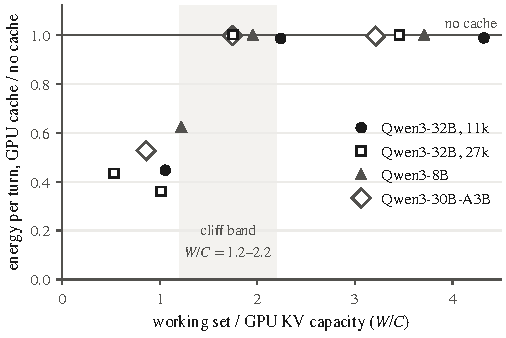
\includegraphics[width=\columnwidth]{../figures/wall.pdf}
\caption{GPU energy per turn with the GPU cache, relative to no cache, against the working set over the GPU's KV
capacity ($W/C$, with $W$ summing each session's largest prompt in the step), for three models and two context
lengths (vLLM, 5\,s pauses). Up to $W/C\approx1.2$ the cache saves 38--64\%; from 1.75 on the ratio is 1 within 2\%
in every case. Shaded: the band $\kappa=1.2$--2.2 in which hits collapse. At $W/C\approx1.75$ the 27k (16 sessions) and 30B-A3B (96 sessions) points coincide.}
\label{fig:wall}
\end{figure}

\paragraph{Eviction policy does not move the cliff.} Replacing LRU with LFU or SLRU left synthetic thrashing unchanged
(within 0.2\% of LRU in energy per turn at 48 and 96 sessions), consistent with the simulation of Lu et~al., in which even next-call-oracle eviction recovered only
1.08--1.18$\times$ LRU's goodput~\cite{lu2026metastability}, and with Liu et~al., who found on production traces from two
companies that 14 eviction algorithms gave little benefit over LRU~\cite{liu2026fancyevict}. On recorded trajectories at 48 sessions both cost 20--28\% more than
LRU.

\paragraph{Real trajectories are gentler.} Recorded SWE-agent sessions share one system prompt and start small. The GPU
cache kept 88\%, 85\% and 68\% of prompt tokens at 16, 48 and 96 sessions and still 72--73\% at 192 and 288, where we
had predicted under 30\%. Our synthetic sessions, with no shared prefix and steady growth, overstate collapse for these
2024 trajectories, whose final contexts are about 12k tokens. Production coding agents now carry far longer contexts
(a median of 68k prompt tokens per call in GitHub Copilot's traces~\cite{copilot2026wild}), which by Eq.~\eqref{eq:cliff} moves
them toward the long-context case above.
